\chapter[Ifi 2]{Kamp nytter! - Prosessen til Ole-Johan Dahls hus}

\label{chap:ifi2}

\author{Skrevet av Narve Trædal}

\begin{figure}
	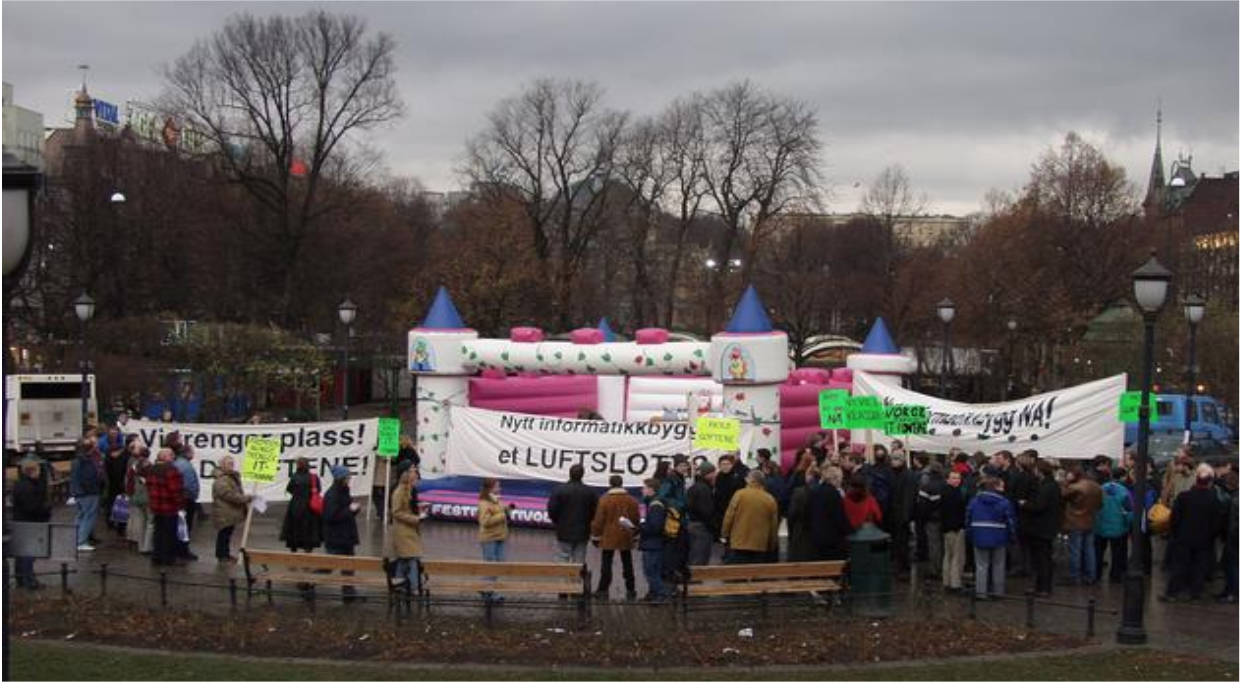
\includegraphics[width=\linewidth]{images/ifi2/hoppeslott.png}
	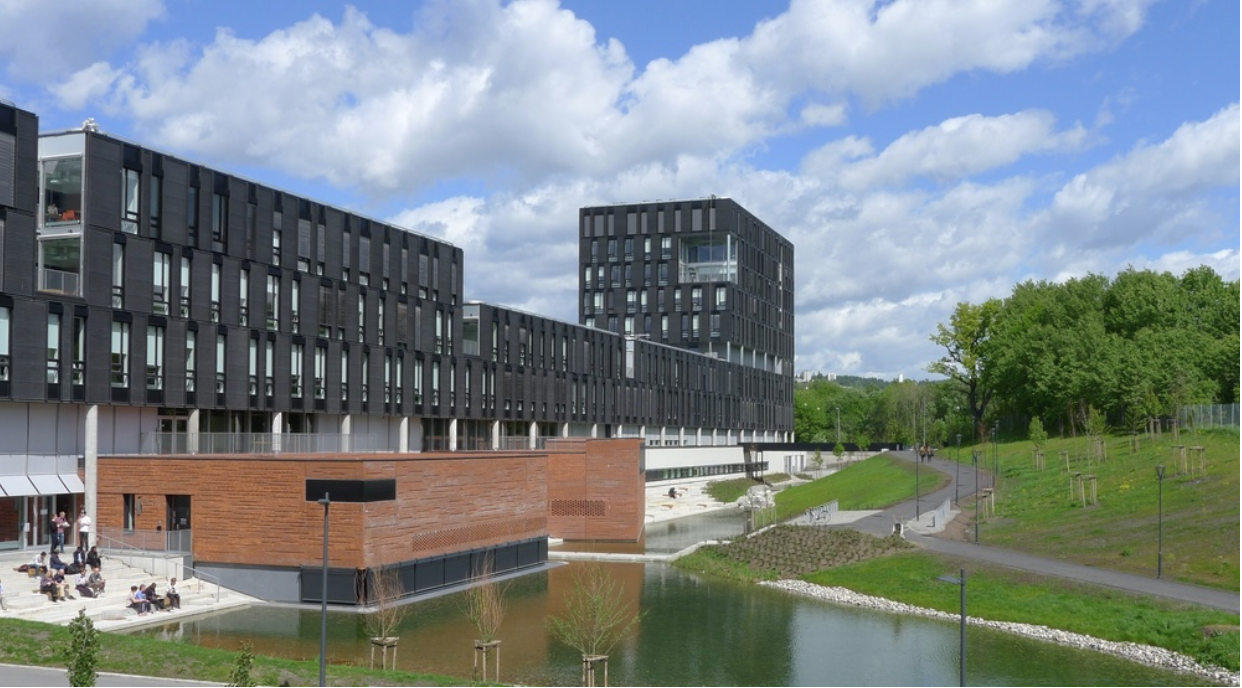
\includegraphics[width=\linewidth]{images/ifi2/ifi2.png}
	\caption{Fra luftslott til Ifi-slott. Et samlet press, og uordodokse aksjoner fra studenter og lærere skapte luftslottet Ifi II om til Ifi-slottet Ole-Johan Dahls hus}
\end{figure}

Helt fra innflyttingen i 1988 var det klart at IT-miljøenes rombehov fortsatt på ingen måte var dekket. Universitetsledelsen tok straks til å tenke på utvidelser et nytt byggetrinn, en ``Informatikkbygningen II'', for å avhjelpe først og fremst IFIs, men også USITs voksende behov. Riktignok var det en dipp i studenttilstrømningen midt på 90-tallet, men dot.com.-bølgen og ``YK2''- engstelsen på slutten av 90-tallet sørget for at samfunnsbehovet for informatikere ble kraftig artikulert i media, og studentene stømmet til på nytt. Men nå var ombyggingsmulighetene i Informatikkbygningen brukt opp, og ``Brakka'' var full.

Da IT-Fornebu-prosessen kom opp på den politiske dagsorden etter midten av 1990-årene, så dukket det på Ifi opp ideer om hvordan romproblemene kunne løses, en gang for alle. Man ønsket å gå radikalt til verks og flytte hele Ifi til nye lokaler på Fornebu. Og gjerne etablere et nytt fakultet der ute med det samme. Ved instituttet var det flere toneangivende stemmer i instituttstyret som så på dette som en spennende løsning. Nye krefter var kommet inn i styre og stell, med bl.a. Aslak Tveito, Morten Dæhlen, Narve Trædal, Kristin Braa og andre fra systemarbeidsmiljøet. Men det var også stor skepsis, særlig blant studentene, men også blant mange ansatte. Deres hovedinnvending var at den geografiske avstanden mellom et Ifi på Fornebu og resten av mat.nat-fakultetet ville være uholdbar for de mange som kombinerte Ifi-emner med andre mat.nat.-emner samme studiesemester.

De to rektorene; Lucy Smith ved UiO, og Emil Spjøtvoll ved NTNU, gikk inn for at det burde etableres en omfattende to-årig hovedfagsutdanning på Fornebu, som et ledd i eit nytt profesjonsstudium i informatikk. Utdanningen skulle føre fram til cand.scient.\slash siv.ing.-utdanning innen informatikk og
kommunikasjonsteknologi med en årsproduksjon på mellom 80 og 160. Utdanningen burde skje i samarbeid med Telenor, som var i ferd med å etablere seg der ute. Mange på Ifi var også skeptiske til dette. De ønsket ikke å dele opp staben og undervisningen på to campus. Men instituttstyret ved Ifi sluttet opp om dette, dog som et klart B-alternativ, dersom det skulle vise seg at hovedalternativet: pånybygging av Informatikkbygningen, eller aller helst et nybygg i Gaustadbekkdalen ikke lot seg realisere.

Resultatet ble at den akademiske aktiviteten på Fornebu, ble definert som en ren forsknings- og veiledningsaktivet, utan ordinær undervisning. Simula Resarch laboratory, til daglig kalt Simula-senteret, ble etablert fra 2001, bemannet i vesentlig grad med ansatte ved Ifi; professorer som stort sett fikk en løpende 80\% permisjon fra sin faste Ifi-stilling.

Studentene sto hele tiden på at den at den eneste akseptable løsningen var nybygging i Gaustadbekkdalen. Fagutvalget for informatikk, FUI, var særlig aktive, og fikk god støtte, bl.a. fra representantar for Systemarbeidsmiljøet, som huset mange ``gamle'' aktivister.

1.oktober 1998 holdt Jens Kaasbøll sin ordinære IN 105-forelesning på ``Dasslokket'' (uteserveringen til Tostrupkjelleren, vis-a-vis Stortinget) kl 14.15, fullt utstyrt med prosjektør og lydanlegg. 200 studenter møtte opp, og i etter å ha fått med seg innholdet i Kaasbølls forelesning, holdt de en punktdemonstrasjon med slagordene:

\begin{itemize}
	\item ``Hold Ifi samlet!''
	\item ``Stopp raseringen av informatikkutdanningen!''
	\item ``Nybygg nå!''
\end{itemize}

Ved siden av aksjonene foregikk det lobbyverksomhet, og bare en måned etter ``Dasslokk-forelesningen'', klarte en delegasjon fra FUI, via eit møte med lederen for KUF-komiteen, samt KUF-minister Jon Lilletun, å få inn en merknad i budsjettforslaget for 1999 om at KUF-komiteen, ``ber Regjeringa legge til rette for at Noregs forskingsråd allereie i 1999 kan starte arbeidet med å utvide det såkalla ``Informatikkbygget'' i Gaustadbekkdalen i Oslo med eit byggetrinn på inntil 10 000 m2.''

Det grunnleggende valget om behov og lokalisering var således nå bestemt på høyeste politiske hold. Og selv om det skulle ta flere frustrerende år før prosjektet nærmet seg startbevilgning, og tilsvarende år med stadig meir omseggripende mer eller mindre provisoriske romløsninger, så var det etter denne komitemerknaden aldri tvil om hva som skulle bli den endelege løsningen på Ifis plassproblemer.

I de nesten sju årene, etter Kaasbølls 105-forelesning, fram til den første byggebevilgningen ble en realitet, og i selve byggetiden, flyttet så studenter og ansatte fortsatt rundt på campus. I 2005 hadde instituttet følgende lokaler utenfor Informatikkbygningen:

\begin{itemize}
	\item Forskningparken I og II
	\item Veilaboratoriet i Gaustadalleen
	\item Preklinisk odontologi-bygningen
	\item Vilhelm Bjerknes hus
	\item Niels Henrik Aabels hus
	\item Sophus Lies auditorium
\end{itemize}

Påvirkningsprosessen fra UiOs side skjedde stort sett ved brev og møter med politikere og departement for å presse fram IFI II-bevilgninger. Men andre aksjonsformer ble fortsatt prøvd. Den mest legendariske er hoppeslott-aksjonen utenfor Stortinget 28.november 2001, da ifi-ansatte og studenter satte opp et hoppeslott, dandert med farger og slagord nedenfor Stortingsbakken, og avholdt en fengende demonstrasjon med paroler og appeller fra både studenter og professorer.

\begin{figure}
	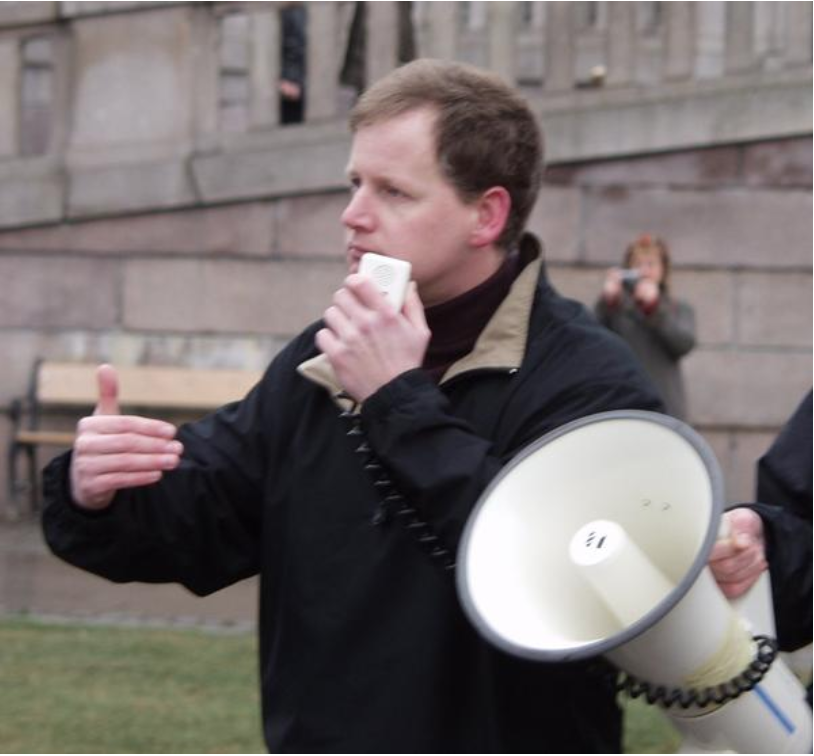
\includegraphics[width=\linewidth]{images/ifi2/knut-yrvin-demonstrasjon.png}
	\caption{Knut Yrvin holder studentappellen under ``hoppeslott-demoen''.}
\end{figure}

\begin{figure}
	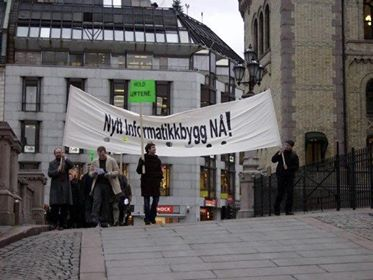
\includegraphics[width=\linewidth]{images/ifi2/ifi2-demonstrasjon.jpg}
	\caption{Demonstrasjon utenfor Stortinget, med blant annet Thomas Fyhn og Petter Hareim i front.}
\end{figure}

Og lobby-virksomheten bar til slutt frukter. Våren 2005, kunne undervisnings- og forskningsminister Kristin Clemet foran et fullsatt Store auditorium i Informatikkbygningen, kunngjøre at startbevilgning var gitt.

Ennå skulle det ta fem lange år før huset sto der. Primus motor for byggeprosessen ved Ifi var Terje Knudsen, leder av Ifis tekniske driftsseksjon. Han viste seg å ha et stort talent for prosjektutvikling i byggesaker, og drog lasset for instituttet, og også i betydelig grad for hele UiO, i den langvarige
byggefasen der både naturen og budsjettrammene var krevende å hanskes med. Men senhøsten 2010 kunne Ifi-drift se de første flyttelassen sige over plassen fra Ifi I til Ifi II, eller fra Kristen Nygaards hus til Ole-Johan Dahls hus, som var blitt deres offisielle navn. Driftsgjengen ved Ifi sto på,
nærmest dag og natt i uker og måneder rundt juletider. Og målet ble nådd: Fra og med vårsemesteret 2011 var all aktivitet samlet i det nye Ifi-slottet. Der alle, både ansatte og studenter; forskning, undervisning og studentaktiviteter, hadde god plass – i et bygg som fikk Oslo kommunes arkitekturpris for 2010, der det ligger som en supertanker, midt i Gaustadbekkdalen, med kurs mot fjorden og mot verden.

Helt smertefritt var likevel ikke innflyttingen. Den automatstyrte romoppvarmingen hadde sine betydelige svakheter, og stipendiatene klaget over dårlig fysisk arbeidsmiljø på sine store åpne kontorarealer. Men etter hvert ble disse svakhetene rettet opp, og bygget fungerer fortsatt, 8 år etter åpningen, omtrent optimalt for de behov den er laget for.

\begin{figure}
	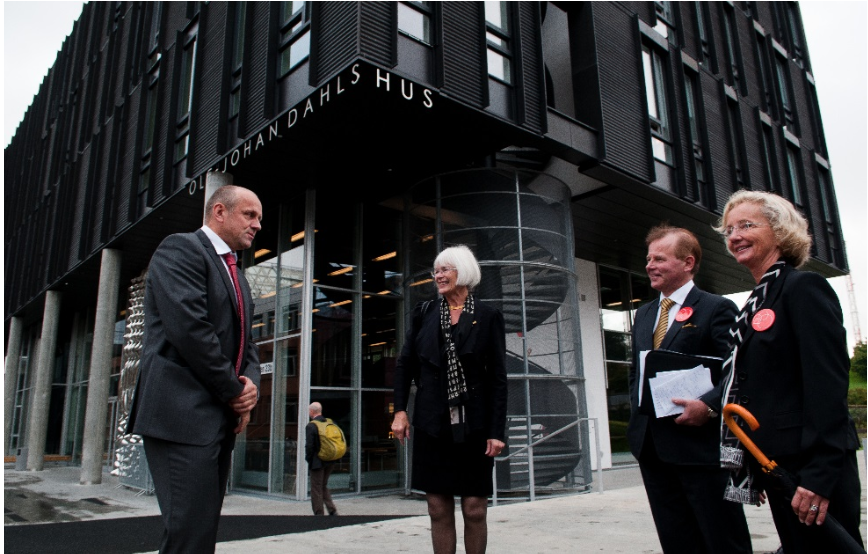
\includegraphics[width=\linewidth]{images/ifi2/ifi2-offisiell-aapning.png}
	\caption{Instituttleder Morten Dæhlen tar imot minister for forsking og høyere utdanning, Tora Aasland, universitetsdirektør Ole Petter Ottersen og universitetsdirektør Gunn-Elin Bjørneboe til den offisielle åpningen på UiOs ``fødselsdag'' 2.september 2011.}
\end{figure}

I tillegg til bygningen fikk Ifi en generøs inventarbevilgning med på kjøpet. Den ble blant annet benyttet til å utstyre instituttets Forskningsgruppe for digitalteknikksystemer med flere og langt mer avanserte laboratorier enn det som var planlagt i utgangspunktet.
